\begin{tcolorbox}
\chapter{2008 --- Votla Gora}

The main focus of the Votla Gora 2008 Expedition to the Tolminski
Migovec plateau, Western Slovenia, was the connection of \passage{Sistem Migovec}
(11493 m - 5\(^{th}\) longest in Slovenia) with \passage{Vrtnarija} (5229 m
- 11\(^{th}\) longest) to make the second longest cave in Slovenia
(16722+m). The separation between the caves was 28 m on the centre line
with many going leads. This was not achieved, but 1.2 km of cave passage
was found and explored.

The part of Sistem Migovec that we were attempting to connect to was the
bottom of \passage{M2}, the original deep cave on Migovec pushed back in
the early 1970s by the Slovenian JSPDT. Below the epic \passage{Tolminski
Silos} pitch (P120 m), the cave shut down into a series of small pitches
with extremely tight rift, which had to be exploded open for passage.
Exploration had finished in the 1970s at yet another such rift.

2008 was also the first ICCC Slovenia expedition with a name - `Votla
Gora', meaning `Hollow Mountain'. This was an idea, shamelessly copied
from the recent OUCC Ario Caves expeditions, which instantly became a
useful tradition.

\end{tcolorbox}
\backgroundsetup{
    scale=1.1,
    color=black,
    opacity=1,
    angle=0,
    contents={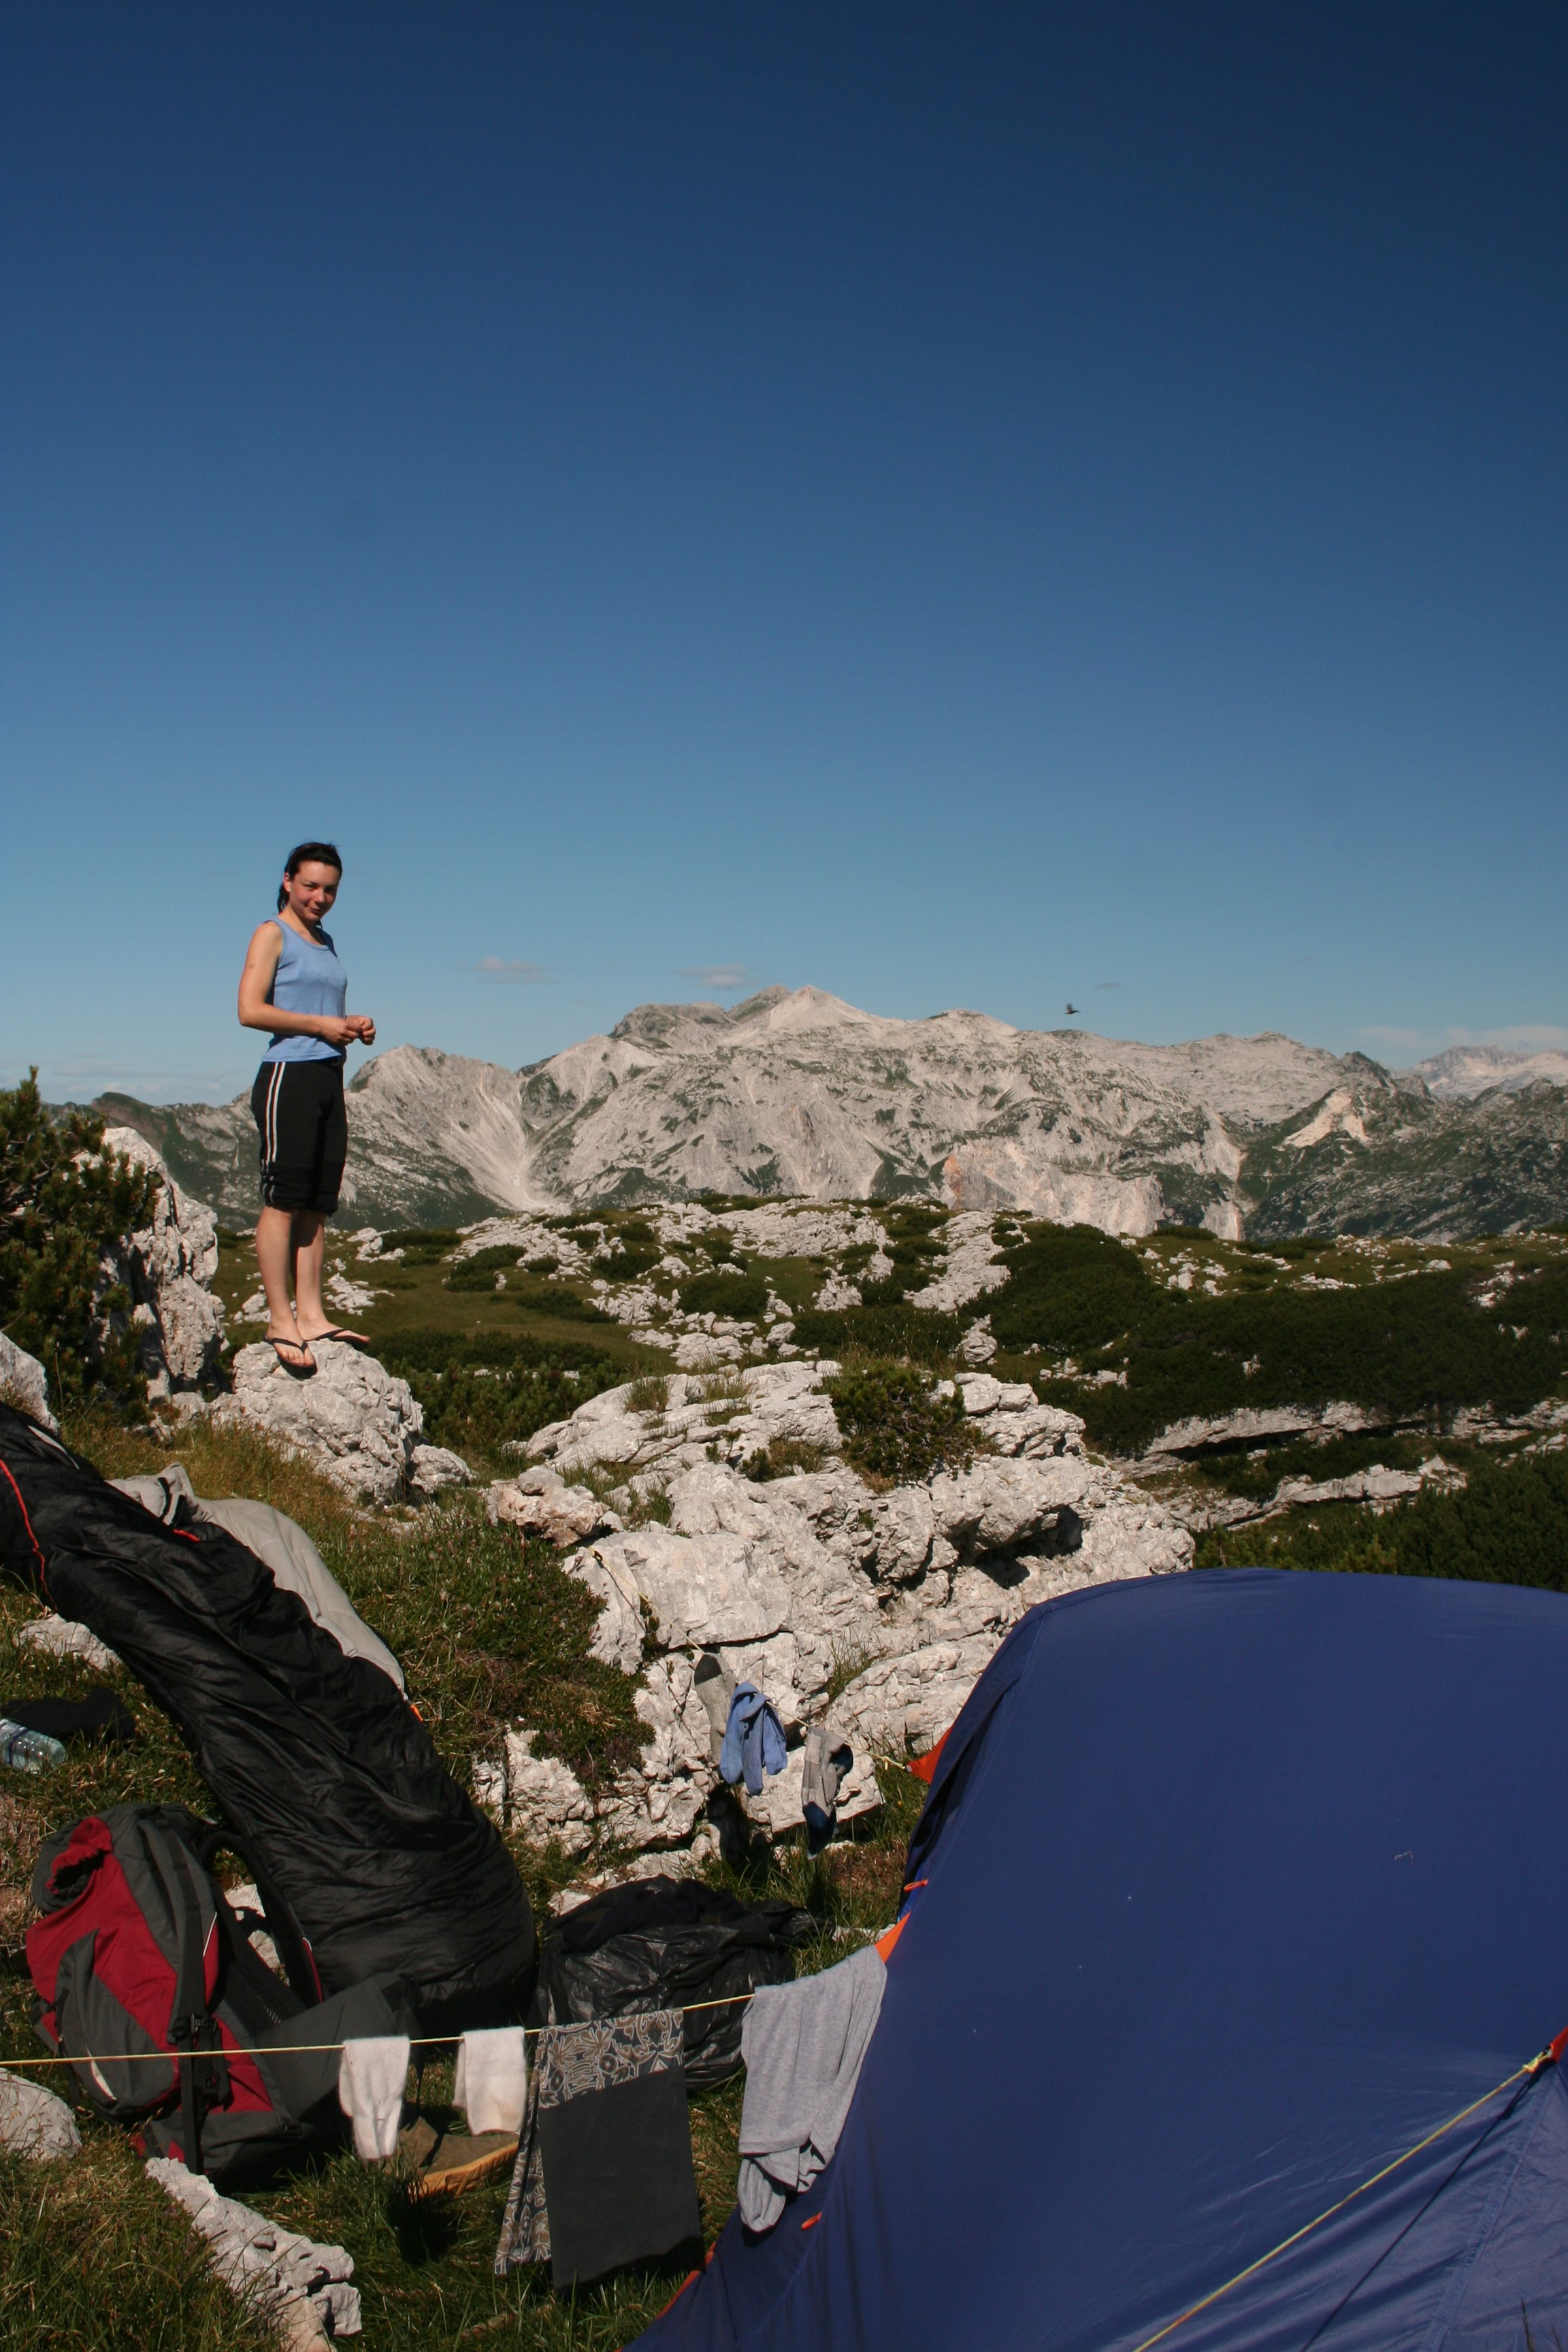
\includegraphics[height=\paperheight]{2008/intro/Jana Carga - Canon 350D - img_2998 jana posed by tent in morning on clear day.jpg}}
}
\BgThispage









